\begin{solution}
\begin{enumerate}
\item {[3 points]} Let $\boldsymbol{\alpha}^{(0)}\in\R^{N+1}$ be the vector with entries $\alpha_j^{(0)}=u_0(x_j)$, let the mass matrix $\BM\in\R^{\left(N+1\right)\times\left(N+1\right)}$ be the matrix with entries
\[
M_{jk}=\int_0^1\phi_k(x)\phi_j(x)\,dx
\]
and let the stiffness matrix $\BK\in\R^{\left(N+1\right)\times\left(N+1\right)}$ be the matrix with entries
\[
K_{jk}=\int_0^1(1+\sin(\pi x))\phi_k'(x)\phi_j'(x)\,dx.
\]
Then $\boldsymbol{\alpha}(t)$ is the solution to the system of ordinary differential equations
\[
\BM\boldsymbol{\alpha}'(t)=-\BK\boldsymbol{\alpha}(t)
\]
with initial condition
\[
\boldsymbol{\alpha}(0)=\boldsymbol{\alpha}^{(0)}.
\]
\\
\item {[3 points]} For $k=1,2,3,\ldots$, we can use the forward Euler method to obtain approximations $\boldsymbol{\alpha}^{(k)}$ to $\boldsymbol{\alpha}(t_k)$. We can compute these approximations as
\[
\boldsymbol{\alpha}^{(k)}=\boldsymbol{\alpha}^{(k-1)}+\Delta t\boldsymbol{\beta}^{(k-1)}
\]
where $\boldsymbol{\beta}^{(k-1)}$ is the solution of
\[
\BM\boldsymbol{\beta}^{(k-1)}=-\BK\boldsymbol{\alpha}^{(k-1)}.
\]
It is also acceptable to say that we can compute $\boldsymbol{\alpha}^{(k)}$ by solving
\[
\BM\boldsymbol{\alpha}^{(k)}=\left(\BM-\Delta t\BK\right)\boldsymbol{\alpha}^{(k-1)}.
\]
\\
\item {[6 points]} The requested plots are below.

\begin{center}
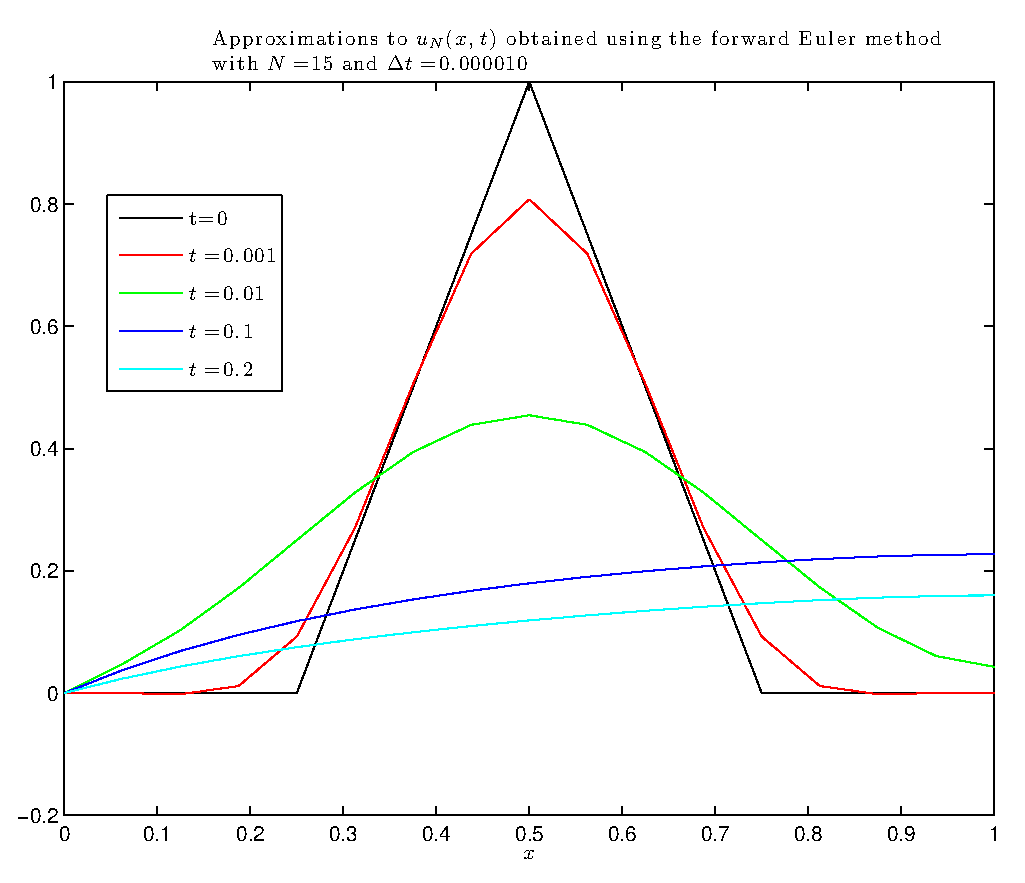
\includegraphics[scale=0.75]{hw50c15.eps}
\end{center}

\begin{center}
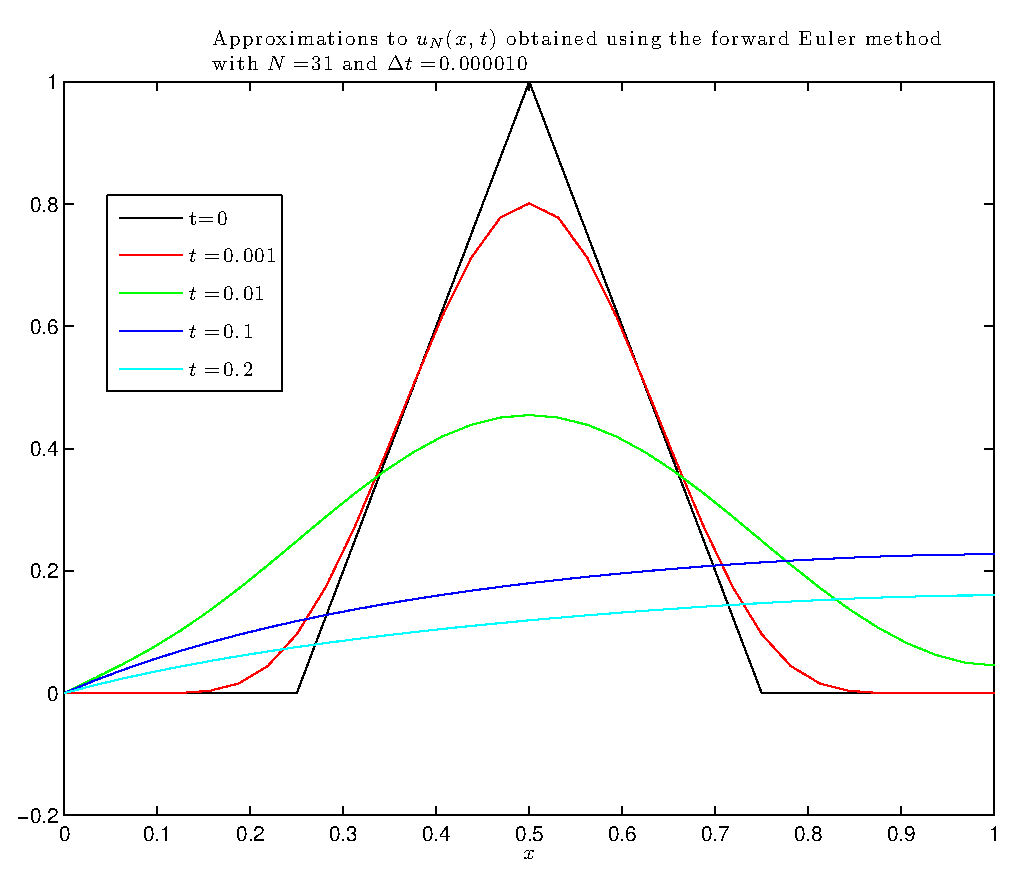
\includegraphics[scale=0.75]{hw50c31.eps}
\end{center}
The code used to produce the results shown in this part and in parts (d) and (f) is below.  Note that the below code uses the MATLAB functions which you had to write in Homework 2 and Homework 49.

\lstinputlisting{HW50.m}

\item {[4 points]} The requested plots are below.

\begin{center}
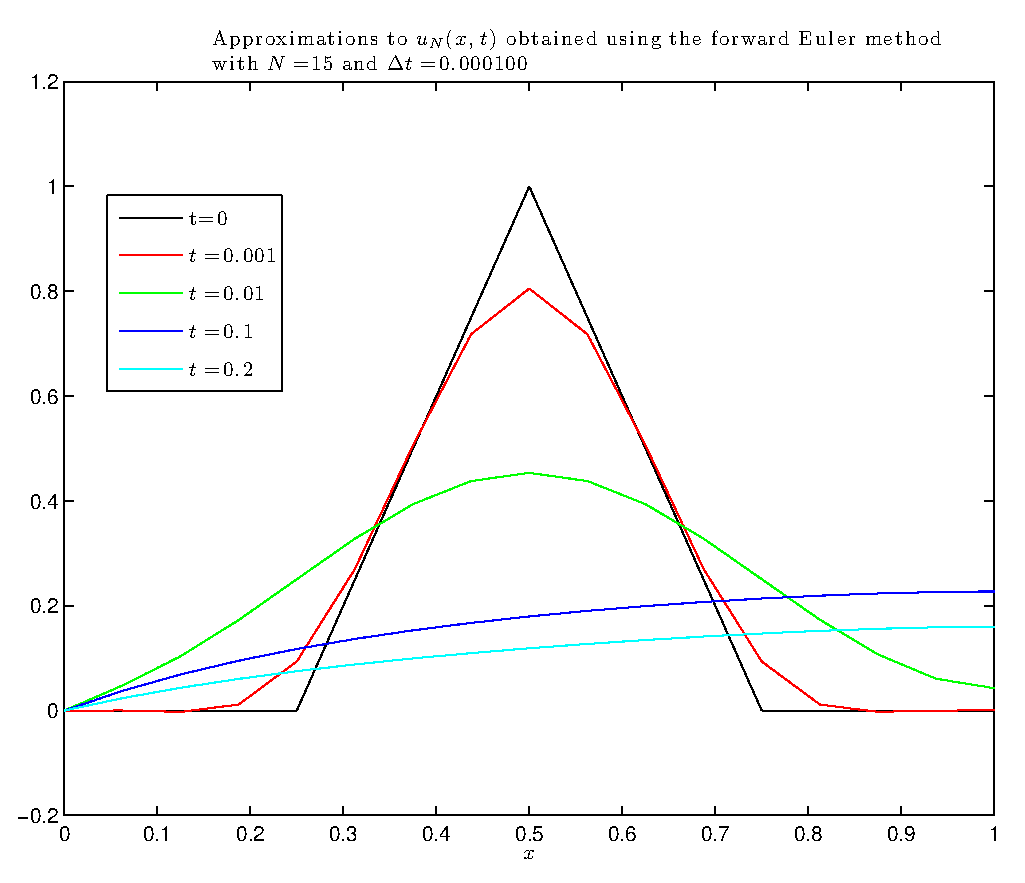
\includegraphics[scale=0.75]{hw50d15.eps}
\end{center}

\begin{center}
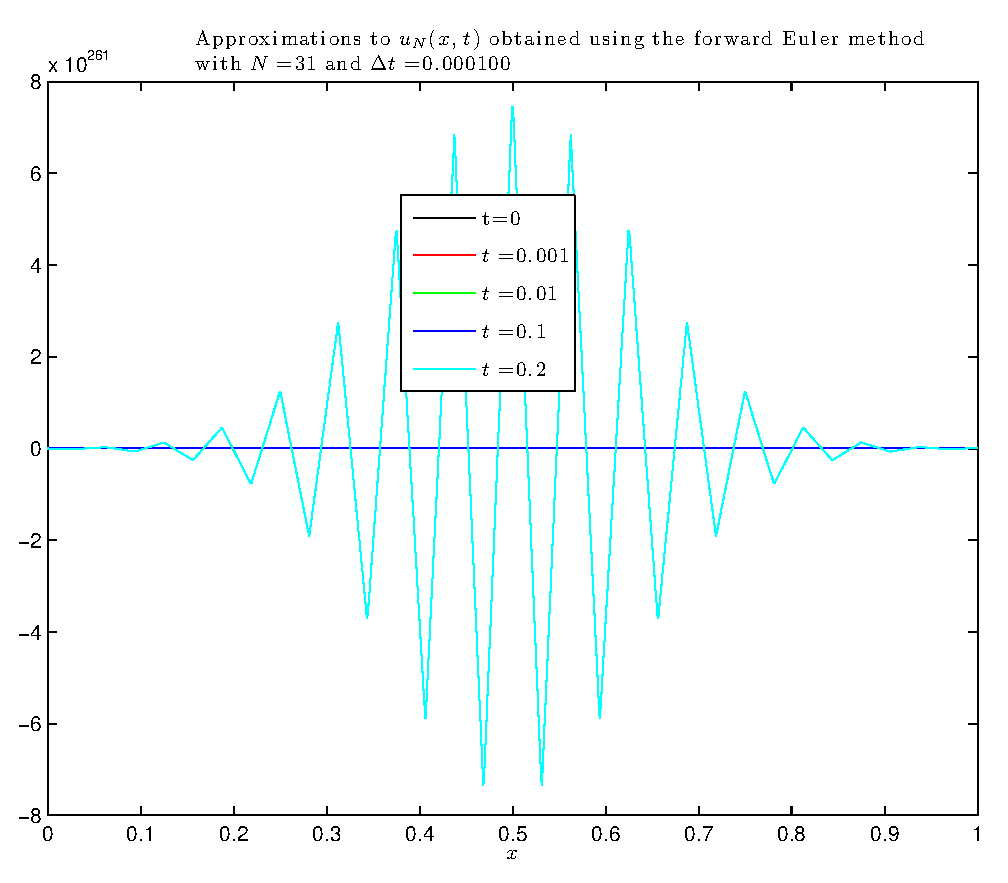
\includegraphics[scale=0.75]{hw50d31.eps}
\end{center}

\item {[3 points]} For $k=1,2,3,\ldots$, we can use the backward Euler method to obtain approximations $\boldsymbol{\alpha}^{(k)}$ to $\boldsymbol{\alpha}(t_k)$. We can compute these approximations by solving
\[
\left(\BM+\Delta t\BK\right)\boldsymbol{\alpha}^{(k)}=\BM\boldsymbol{\alpha}^{(k-1)}.
\]

\item {[6 points]} The requested plots are below.

\begin{center}
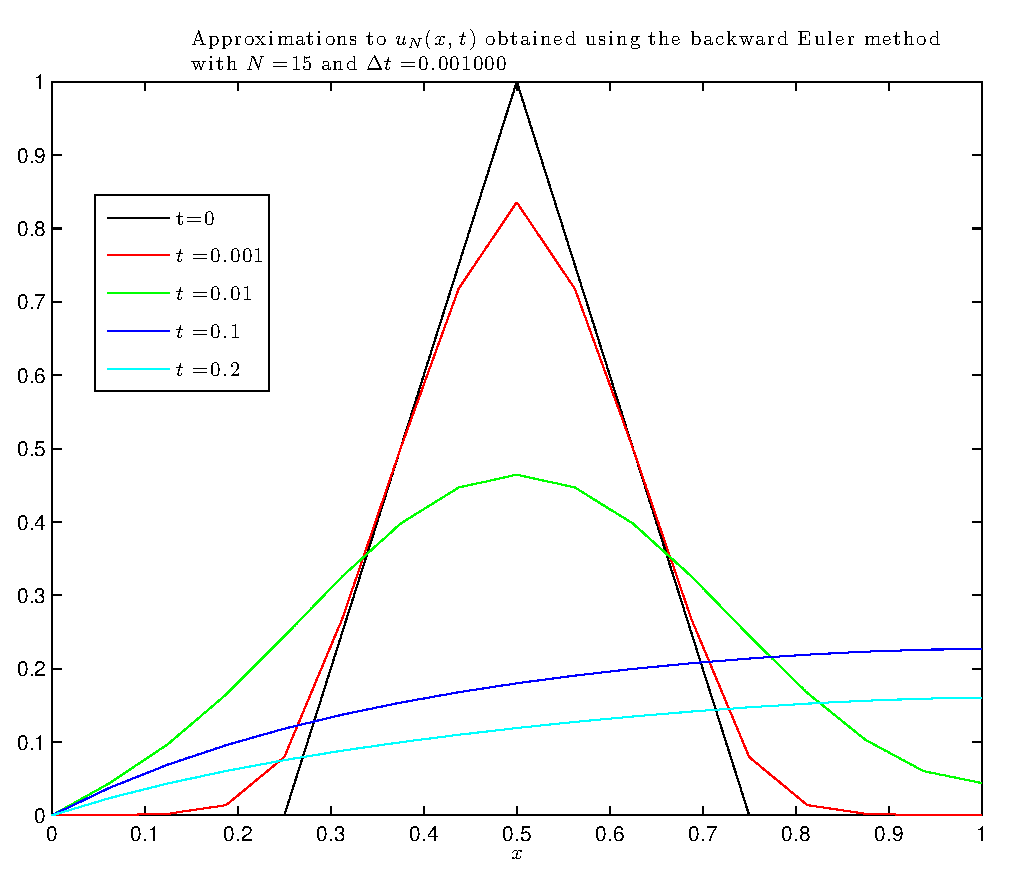
\includegraphics[scale=0.75]{hw50f15.eps}
\end{center}

\begin{center}
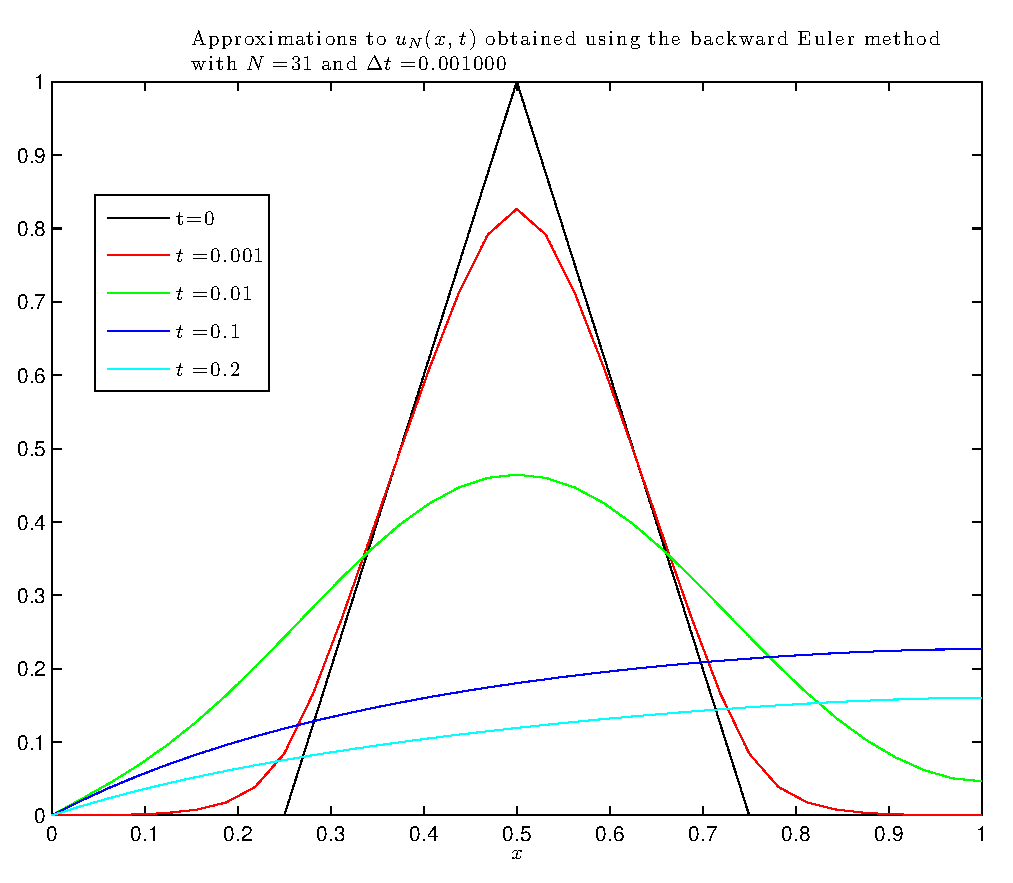
\includegraphics[scale=0.75]{hw50f31.eps}
\end{center}

\end{enumerate}
\end{solution}